\documentclass[12pt, openany]{report}
\usepackage[utf8]{inputenc}
\usepackage[T1]{fontenc}
\usepackage{amsmath,amsfonts,amssymb}
\usepackage{amssymb}
\usepackage{multicol}
\usepackage[a4paper,left=2.5cm,right=2.5cm,top=2.5cm,bottom=2.5cm]{geometry}
\usepackage[english]{babel}
\usepackage{libertine}
\usepackage{graphicx}
\usepackage{wrapfig}
\usepackage{algorithm}
\usepackage{algpseudocode}
\usepackage{float}
\usepackage{enumitem}
\usepackage{pythonhighlight}
\usepackage[]{titletoc}
\usepackage{empheq}
\usepackage{titlesec}
\usepackage{mathpazo}
\usepackage{xfrac}
\usepackage{textcomp}
\usepackage{mathtools}
\usepackage{caption}
\usepackage{tabularray}
\usepackage{subcaption}
\usepackage{cancel}
\usepackage[bottom]{footmisc}
\usepackage{pdfpages}
\usepackage{tabularx}
\usepackage{amsthm}
\usepackage[skins]{tcolorbox}
\titleformat{\chapter}[display]
  {\normalfont\bfseries}{}{0pt}{\Huge}
\usepackage{hyperref}
\newcommand{\hsp}{\hspace{20pt}}
\newcommand{\HRule}{\rule{\linewidth}{0.5mm}}
\newcommand{\R}{\mathbb{R}}
\newcommand{\C}{\mathcal{C}}
\renewcommand{\O}{\mathcal{O}}
\theoremstyle{definition}
\newtheorem{thm}{Theorem}[chapter]
\newtheorem{definition}[thm]{Definition}
\newtheorem{lem}[thm]{Lemma}

\hbadness=100000
\begin{document}
\begin{titlepage}
    \begin{sffamily}
    \begin{center}
        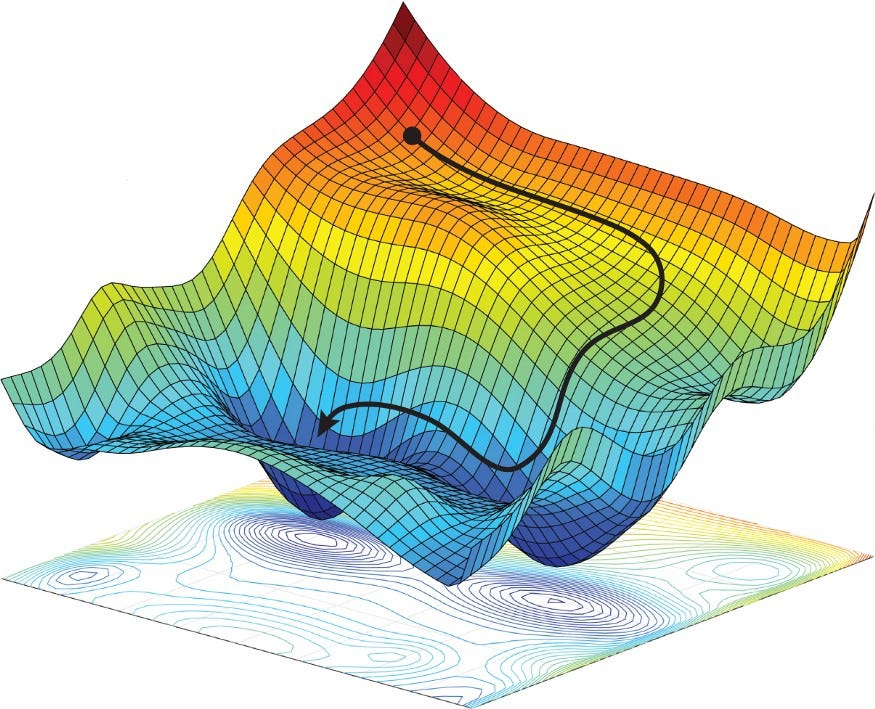
\includegraphics[scale=0.3]{img/page_de_garde.png} \\[1cm]
        \HRule \\[0.4cm]
        { \huge \bfseries LINMA2460 Nonlinear Programming \\[0.4cm] }
    
        \HRule \\[1.5cm]
        \textsc{\LARGE Simon Desmidt\\ Issambre L'Hermite Dumont}\\[1cm]
        \vfill
        \vspace{2cm}
        {\large Academic year 2024-2025 - Q2}
        \vspace{0.4cm}
         
        
\includegraphics[width=0.15\textwidth]{img/epl.png}
        
        UCLouvain\\
    
    \end{center}
    \end{sffamily}
\end{titlepage}

\setcounter{tocdepth}{1}
\tableofcontents
\chapter{Definitions, notations and random properties}
\begin{itemize}
	\item The Taylor expansion of order $p$ of the function $f$ around $x_k$ and evaluated at $y$ is: 
	\begin{equation}
		T_p(y;x_k) = f(x_k) + \sum_{i=1}^{p} \frac{1}{i!} D^i f(x_k) (y-x_k)^i
	\end{equation}
	\item We can thus define the gradient w.r.t. $y$ of the Taylor expansion of order $p$ of $f$ around $x_k$ and evaluated at $x_{k+1}$:
	\begin{equation}
		\nabla_y T_p(x_{k+1};x_k) = \left. \nabla_y T_p(y;x_k) \right|_{y=x_{k+1}}
	\end{equation}
	\item An oracle is a "black box" that gives information about the derivatives based on $x$. The general form of an oracle is:
	\begin{equation}
		\text{p-order oracle:} \quad x \mapsto \{D^if(x)\}_{i=0}^p
	\end{equation}
	And so we have the following simple oracles examples:
	\begin{equation}
		\begin{aligned}
			\text{Zero}^{th} \text{-order oracle:} \quad &x \mapsto \{f(x)\} \\
			\text{First-order oracle:} \quad &x \mapsto \{ f(x), \nabla f(x) \} \\
			\text{Second-order oracle:} \quad &x \mapsto \{ f(x), \nabla f(x), \nabla^2 f(x) \}
		\end{aligned}
	\end{equation}
    \item $\C^p_L(\R^n)$: Class of functions p-times continuously differentiable with L-Lipschitz continuous p-order derivative, i.e. $\| D^pf(x) - D^pf(y) \| \leq L \|x-y \|$, $\forall x,y\in \R^n$. And so we have the following simple classes of problems:
    \begin{itemize}
		\item $\C^1_L(\R^n)$: Class of continuously differentiable functions with L-Lipschitz gradient;
    \item $\C^2_L(\R^n)$: Class of continuously differentiable functions with L-Lipschitz hessian.
	\end{itemize}
	\item  p order method (generalization of GM):
	\begin{equation}
		x_{k+1} = \arg\min_{y\in \R^n} \Omega_{x_k,y,p}(y) \equiv T_{x_k,p}(y) + \frac{M}{(p+1)!}\|y-x_k\|^{p+1}
	\end{equation}
\end{itemize}
\section{Properties}
\begin{itemize}
	\item For a function $f\in \C^1(\Omega)$ and $\Omega$ is bounded, the following holds: $\lVert \nabla f(x)\rVert \le L$ for all $x\in \Omega$ for some $L\ge 0$.
	\item By the mean value theorem, for a continuously differentiable function $f$, $\forall x,y\in \Omega,\: \exists \ z\in \Omega:$ $f(y)-f(x) = \langle \nabla f(z),y-x\rangle$.
	\item For a matrix $A$ and a scalar $b$, $\lVert A\rVert \le b\Longrightarrow |\lambda (A)|\le b \Longrightarrow |A| \preceq bI_n$, where the absolute value of the matrix is taken component wise. 
\end{itemize}
\section{Complexity table}
\begin{center}
	\begin{tabular}{|c|c|c|c|c|c|}
		\hline
		Method & Lipschitz & $\nabla f$ & $\nabla^2 f$ & \dots & $\nabla^p f$ \\
		\hline
		Zero order & & $O(n\epsilon^{-2})$ & & & \\
		\hline
		First order & $p=1$ & $O(\epsilon^{-2})$ & & & \\
		\hline
		Second order & $p=2$ & \textcolor{red}{\cancel{X}} & $O(\epsilon^{-3/2})$ & & \\
		\hline
		\vdots & & \textcolor{red}{\cancel{X}} & \textcolor{red}{\cancel{X}} & $\ddots$ & \\
		\hline
		p order & & \textcolor{red}{\cancel{X}} & \textcolor{red}{\cancel{X}} & \textcolor{red}{\cancel{X}} & $O(\epsilon^{-\frac{p+1}{p}})$ \\
		\hline
	\end{tabular}
\end{center}
\chapter{TODO}
We can generalise the property of a L-Lipschitz function to $f\in \C_L^p(\R^n)$. For $p=1$, we had 
\begin{equation}
	f(y)\le f(x_k) + \langle \nabla f(x_k),y-x_k\rangle + \frac{L}{2}\lVert y-x_k\rVert^2 \qquad \forall y\in \R^n 
\end{equation}
For a general value of $p$, it becomes 
\begin{equation}
	f(y) \le T_p(y;x_k) + \frac{L}{(p+1)!}\lVert y-x_k\rVert^{p+1} \qquad \forall y\in \R^n 
\end{equation}
Using this, \textcolor{blue}{we need a $p$-th order oracle} for the method to work. \\
To solve $\min_{x\in \R^n} f(x)$, we can use the iteration 
\begin{equation}\label{eq:argmin}
	x_{k+1} = \arg\min_{y\in \R^n} T_p(y;x_k)+\frac{M}{(p+1)!}\lVert y-x_k\rVert^{p+1}
\end{equation}
where the constant $M$ is an approximation of the Lipschitz constant $L$. \textcolor{blue}{Assuming $f\in \C^p_L(\R^n)$}, we have 
\begin{equation}
	\begin{aligned}
		f(x_{k+1}) &\le T_p(x_{k+1};x_k) + \frac{L}{(p+1)!}\lVert x_{k+1}-x_k\rVert^{p+1}\\
		&= \underbrace{T_p(x_{k+1};x_k) + \frac{M}{(p+1)!}\lVert x_{k+1}-x_k\rVert^{p+1}}_{\le f(x_k)} + \frac{(L-M)}{(p+1)!}\lVert x_{k+1}-x_k\rVert^{p+1}
	\end{aligned}
\end{equation}
where the inequality $\le f(x_k)$ is due to the decrease of $f$ and equation \eqref{eq:argmin}. 
\textcolor{blue}{Suppose that $M>2L$}. After some algebraic manipulations, we get
\begin{equation}\label{eq:bound}
	f(x_k)-f(x_{k+1}) \ge \frac{L}{(p+1)!}\lVert x_{k+1}-x_k\rVert^{p+1}
\end{equation}
On the other hand, using the triangular inequality, 
\begin{equation}
	\begin{aligned}
		\lVert \nabla f(x_{k+1})\rVert & \le \lVert \nabla f(x_{k+1})-\nabla_y T_p(x_{k+1};x_k)\lVert\\
		& + \underbrace{\left \lVert \nabla_y T_p(x_{k+1};x_k)\textcolor{red}{+}\nabla \left.\left(\frac{M}{(p+1)!} \lVert \cdot -x_k\rVert^{p+1}\right)\right|_{y=x_{k+1}}\right \rVert}_{=0}	\\
		& + \left\lVert \nabla \left.\left(\frac{M}{(p+1)!}\lVert \cdot -x_k\rVert^{p+1}\right)\right|_{y=x_{k+1}}\right \rVert \\
		& \le \frac{L}{p!}\lVert x_{k+1}-x_k\rVert^p + \frac{M}{p!} \lVert x_{k+1}-x_k\rVert^p
	\end{aligned}
\end{equation}
\textcolor{red}{Le + rouge doit être un -?}
\begin{equation}\label{eq:bound_on_x}
	\Longrightarrow \lVert x_{k+1}-x_k\rVert \ge \left(\frac{p!}{L+M}\right)^{1/p}\lVert \nabla f(x_{k+1})\rVert^{1/p}
\end{equation}
Combining equations \eqref{eq:bound} and \eqref{eq:bound_on_x}, 
\begin{equation}\label{eq:next_bound}
	f(x_k)-f(x_{k+1}) \ge \underbrace{\frac{L}{(p+1)!}\left(\frac{p!}{L+M}\right)^{\frac{p+1}{p}}}_{\eqcolon C(L)} \lVert \nabla f(x_{k+1})\rVert^{\frac{p+1}{p}}
\end{equation}
Let $T(\varepsilon) = \inf \{k\in \mathbb{N}:\: \lVert \nabla f(x_k)\rVert\le \varepsilon\}$. \textcolor{blue}{Assume that $T(\varepsilon)\ge 2$ and $f(x)\ge f_{low}$ $\forall x\in \R^n$.} Summing up \eqref{eq:next_bound} for $k=0,\dots, T(\varepsilon)-2$,
\begin{equation}
	\begin{aligned}
		f(x_0)-f_{low} &\ge f(x_0)-f(x_{T(\varepsilon)-1}) = \sum_{k=0}^{T(\varepsilon)-2} f(x_k)-f(x_{k+1}) \\ 
		& \ge (T(\varepsilon)-1)C(L) \varepsilon^{\frac{p+1}{p}}\\
		\Longrightarrow T(\varepsilon) &\le 1 + \frac{f(x_0)-f_{low}}{C(L)} \varepsilon^{-\frac{p+1}{p}} \equiv \O\left(\varepsilon^{-\frac{p+1}{p}}\right)
	\end{aligned}
\end{equation}
\chapter{Gradient descent without gradient}
For this problem consider an adversarial attack on block-based image classifier. We have a machine learning model that given an image $a\in\R^p$ it return $c(a)\in\R^m$, where $c_j(a) \in [0,1]$ is the probability of image $a$ to be in class $j$. The classifier prediction is: $j(a) = \arg\max_{j\in [1,\dots,m]} c_j(a)$.
\end{document}